\chapter{Asking Billionaire Women How They Got RICH!}

This chapter is best read as a sequence of commercial constructions rather than a pile of street interviews. We begin with scale before explanation, because that is how the lecture begins: first the jolt, then the search, then the mechanism. From Beverly Hills to Atlanta, the episode keeps returning to the same hard questions. Where does wealth actually sit? How is it protected? How is it compounded? When should a founder keep control, and when does that control become the whole game? The mathematics here is deliberately modest. We write down only those relations that the lecture itself supports, and we treat the rest as cautious reconstruction.

\section{Scale Before Explanation}

The lecture opens by withholding explanation and giving us magnitude. A question about becoming a millionaire is answered by a claim to billionaire status, and then by a claimed peak annual income so large that it functions less as bookkeeping than as a shock to the scale of the page:
\begin{equation}
Y_{\max} \approx \$1.2 \times 10^{9}.
\end{equation}
This quantity is self-reported and should stay that way in our notes. But its role is clear. The lecture wants us to feel the size of the thing before it tells us what to do with it.

The next move is equally important. Instead of immediately teaching a rule, the host reframes the episode as a search. Beverly Hills is the first field. Atlanta is the second. Sarah Blakely is the promised culminating case. The order matters. We are not yet in the doctrine. We are in the setup that justifies the doctrine.

And the first explicit question after the scale shock is already the right one: where do the wealthiest people put their money? The lecture lets that question hang in the air. The answer will arrive later, after we have seen enough of the terrain for the arithmetic to mean something.

\section{Beverly Hills as a Field of Partial Access}

The first Beverly Hills encounter matters because it fails. A producer hints at large revenue and then disappears. The transcript in that moment is unstable enough that we should not build mathematics out of it. But narratively the beat is essential. Wealth is present; access to mechanism is not guaranteed. The lecture is telling us, before it tells us anything else, that proximity to success does not yet amount to understanding.

Only after this false start does the lecture land on a more usable case: a woman from finance who says, in compressed form, that one should invest in what one understands. When pressed for the vehicle, she answers real estate. When pressed again, she narrows to residential. Time and geography enter quickly: her buying goes back to the 1990s, and she distinguishes coastal property from the tax logic of red states.

\paragraph{Anecdote.} We move from a missed interview to a sharper one, and that movement is itself instructive. The lecture is not delivering prepackaged lessons; it is extracting them case by case.

\paragraph{Claim.} Assets should be understandable to their owner. Here the preferred understandable asset is residential real estate.

\paragraph{Mechanism.} The point is not merely that the asset appreciates. The point is that the owner knows what she owns, can hold it over time, and can combine it with deliberate legal structure.

This same interview also includes pointed remarks about hiring, trust, and temperament. Those remarks should remain attributed to the speaker rather than elevated into general law. The durable content lies elsewhere: intelligible assets, long horizons, and structure.

\section{Real Estate, LLCs, and the Protective Shell}

Now the lecture narrows. It is no longer enough to own real estate; we are asked how the ownership is carried. The speaker says that she uses one LLC per property and that the count exceeds fifty. She calls the LLC a veil of protection. The host immediately generalizes: billionaires structure everything.

In the lightest possible notation, we can write the structural move as
\begin{equation}
P_i \mapsto L_i,
\end{equation}
where \(P_i\) is the \(i\)-th property or business asset and \(L_i\) is the LLC shell that carries it. The count given in the interview is
\begin{equation}
N_{\mathrm{LLC}} > 50.
\end{equation}
This is not a legal theorem written on a board. It is a transcript-backed economic schematic. But it is exactly the sort of schematic the lecture invites us to make.

\subsection{Question \& Answer}

\paragraph{Question.} Why put each property in its own LLC rather than holding everything directly?

\paragraph{Answer.} Because the lecture is thinking in compartments. If every asset sits inside the same exposed owner balance sheet, the portfolio behaves like one undivided block. If each asset sits in its own shell, exposure is localized. That is what the phrase veil of protection is doing here. It is translating a legal form into a commercial intuition: structure is part of wealth.

\begin{figure}[h]
\centering
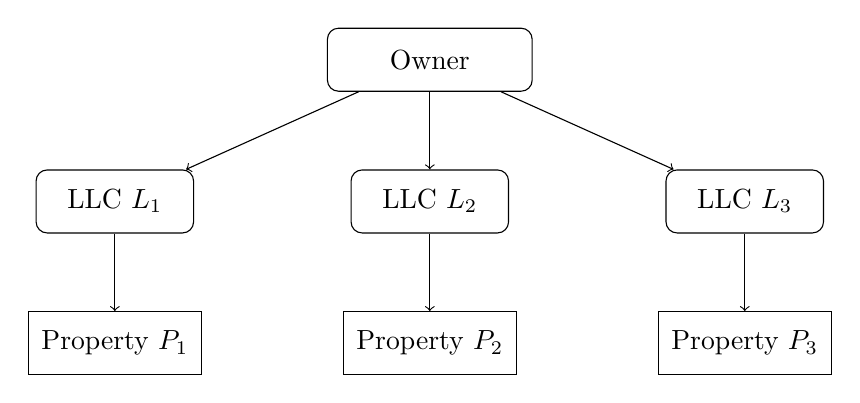
\begin{tikzpicture}[x=1cm,y=1cm]
\node[draw, rounded corners, minimum width=2.6cm, minimum height=0.8cm] (owner) at (0,4) {Owner};
\node[draw, rounded corners, minimum width=2.0cm, minimum height=0.8cm] (llc1) at (-4,2.2) {LLC \(L_1\)};
\node[draw, rounded corners, minimum width=2.0cm, minimum height=0.8cm] (llc2) at (0,2.2) {LLC \(L_2\)};
\node[draw, rounded corners, minimum width=2.0cm, minimum height=0.8cm] (llc3) at (4,2.2) {LLC \(L_3\)};
\node[draw, minimum width=2.2cm, minimum height=0.8cm] (p1) at (-4,0.4) {Property \(P_1\)};
\node[draw, minimum width=2.2cm, minimum height=0.8cm] (p2) at (0,0.4) {Property \(P_2\)};
\node[draw, minimum width=2.2cm, minimum height=0.8cm] (p3) at (4,0.4) {Property \(P_3\)};
\draw[->] (owner) -- (llc1);
\draw[->] (owner) -- (llc2);
\draw[->] (owner) -- (llc3);
\draw[->] (llc1) -- (p1);
\draw[->] (llc2) -- (p2);
\draw[->] (llc3) -- (p3);
\end{tikzpicture}
\caption{Transcript-backed reconstruction of the lecture's liability-shell logic: ownership is layered through separate entities rather than pooled into one exposed block.}
\end{figure}

The lecture pauses here for a sponsor detour, and that pause is worth noting. It shows the host translating one technical practice into a broader entrepreneurial slogan. Still, the durable content is simple: the rich do not merely buy assets; they decide what legal container will carry them.

\section{Ownership Without Dilution: The Beauty Founder Machine}

The next case is the first one that behaves like a full operating machine rather than a street fragment. A Beverly Hills beauty founder says she started in 1997, came from Romania under a communist regime, arrived without money, language, or network, and later sold a company that she still describes as entirely hers before sale:
\begin{equation}
t_0 = 1997,\qquad t_s = 2018,\qquad s_f = 1,\qquad V_{\mathrm{beauty}} \approx \$3 \times 10^{9}.
\end{equation}
The valuation language in the transcript is a little rough, so \(V_{\mathrm{beauty}}\) should stay approximate. But the ownership claim \(s_f=1\) is central. No outside investors stand between founder and firm.

The lecture then slows down and becomes financially explicit. Her advice is to watch cash flow, to care about profit, and to keep personal spending subordinate to the business. The natural way to summarize the logic is with a retained-capital update:
\begin{equation}
K_{t+1} = K_t + \Pi_t - D_t.
\end{equation}
Here \(K_t\) is business capital, \(\Pi_t\) is operating surplus in a broad transcript-backed sense, and \(D_t\) is owner draw. The sign pattern is the point. The interview is not teaching accounting detail. It is teaching direction: keep \(D_t\) small enough that the firm can thicken.

The lecture makes that point concrete by way of restraint rather than glamour:
\begin{equation}
C_{\mathrm{car}} \approx \$200.
\end{equation}
That figure matters symbolically, not financially. It marks the refusal to let appearance outrun accumulation.

\paragraph{Anecdote.} A founder drives a battered car, ignores social embarrassment, and recycles generated money back into the business.

\paragraph{Claim.} Cash flow matters more than lifestyle display.

\paragraph{Mechanism.} When retained capital thickens, the business can finance its own expansion instead of waiting for outside permission.

\subsection{Question \& Answer}

\paragraph{Question.} If we keep reinvesting, how does that actually become scale rather than mere repetition?

\paragraph{Answer.} The lecture answers by sequencing the business. First cash flow. Then more product. Then wider distribution. Then, if the founder is alert, a new channel that changes the geometry of the firm:
\begin{equation}
\text{cash flow} \rightarrow \text{production} \rightarrow \text{distribution widening} \rightarrow \text{brand scale}.
\end{equation}

And now the lecture adds the decisive pivot. Around 2012, her daughter proposes Instagram as a substitute for constant travel. The company posts products, gets into the hands of artists and creators, benefits from tutorials and platform visibility, and the business ``explodes.'' In schematic form,
\begin{equation}
\text{travel-heavy promotion} \rightarrow \text{platform visibility} \rightarrow \text{viral proof} \rightarrow \text{distribution acceleration}.
\end{equation}

\begin{figure}[h]
\centering
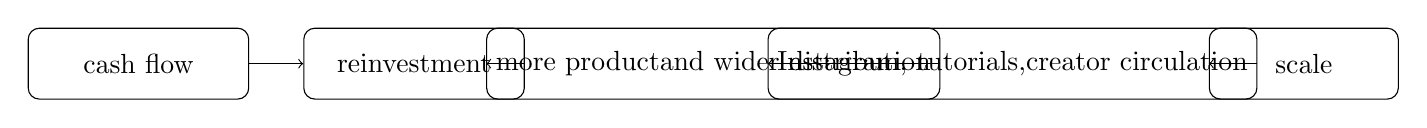
\begin{tikzpicture}[x=1cm,y=1cm]
\node[draw, rounded corners, minimum width=2.8cm, minimum height=0.9cm] (cf) at (-6,0) {cash flow};
\node[draw, rounded corners, minimum width=2.8cm, minimum height=0.9cm] (re) at (-2.5,0) {reinvestment};
\node[draw, rounded corners, minimum width=3.0cm, minimum height=0.9cm] (pd) at (1.3,0) {more product\\and wider distribution};
\node[draw, rounded corners, minimum width=3.0cm, minimum height=0.9cm] (ig) at (5.1,0) {Instagram, tutorials,\\creator circulation};
\node[draw, rounded corners, minimum width=2.4cm, minimum height=0.9cm] (sc) at (8.8,0) {scale};
\draw[->] (cf) -- (re);
\draw[->] (re) -- (pd);
\draw[->] (pd) -- (ig);
\draw[->] (ig) -- (sc);
\end{tikzpicture}
\caption{Transcript-backed reconstruction of the beauty founder's scaling path: retained cash first, then distribution, then platform amplification.}
\end{figure}

This is also where the lecture broadens its temporal horizon. The founder says one must keep adapting; what changed the game once will not remain the last change. She explicitly extends the principle from Instagram to AI. The governing idea is not technological fashion. It is alertness.

And then, after the machinery of reinvestment and scaling, the lecture makes one of its most careful philosophical corrections: money buys freedom, not fulfillment. This does not cancel the business arithmetic. It tells us what that arithmetic can and cannot purchase.

\section{Atlanta: Portfolio Math and the Anti-Cash Rule}

The lecture now leaves Beverly Hills. That travel beat is not decorative. It resets the ear and tells us that we are entering a new money grammar. Atlanta is announced not just as another wealthy city, but as the city through which the Sarah Blakely case will become reachable. Before that culmination, however, the lecture gives us its cleanest explicit arithmetic.

A Wall Street-to-tech founder describes a typical wealth split among the richest people she has observed:
\begin{align}
W &= W_{\mathrm{mkt}} + W_{\mathrm{cash}} + W_{\mathrm{alt}}, \\
W_{\mathrm{mkt}} &= 0.8W, \qquad
W_{\mathrm{cash}} = 0.1W, \qquad
W_{\mathrm{alt}} = 0.1W.
\end{align}
The transcript supplies the compartments. Marketable securities mean stocks, bonds, mutual funds, and ETFs. Alternatives mean illiquid investments such as real estate and private deals. The latter are not for instant access but for a longer compounding interval:
\begin{equation}
T_{\mathrm{alt}} \in [5,10]\ \text{years}.
\end{equation}

\begin{figure}[h]
\centering
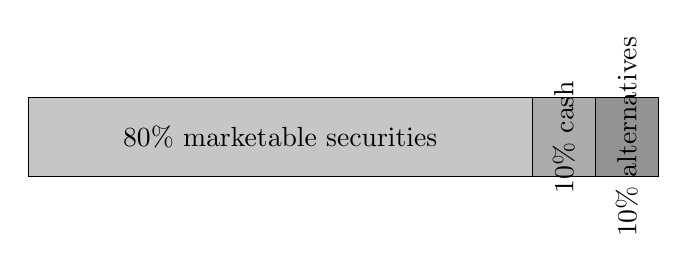
\begin{tikzpicture}[x=1cm,y=1cm]
\draw[fill=gray!20] (0,0) rectangle (8,1);
\draw[fill=gray!45] (0,0) rectangle (6.4,1);
\draw[fill=gray!65] (6.4,0) rectangle (7.2,1);
\draw[fill=gray!85] (7.2,0) rectangle (8,1);
\node at (3.2,0.5) {\(80\%\) marketable securities};
\node[rotate=90] at (6.8,0.5) {\(10\%\) cash};
\node[rotate=90] at (7.6,0.5) {\(10\%\) alternatives};
\end{tikzpicture}
\caption{Transcript-backed reconstruction of the lecture's allocation rule. The precise percentages are speaker-supplied; the bar is an interpretive aid.}
\end{figure}

\subsection{Question \& Answer}

\paragraph{Question.} Where do the richest people actually put their money, and why not leave it in cash?

\paragraph{Answer.} Because the lecture's governing metaphor is that money should have a job. Cash exists, but it is not the dominant form in which wealth lives. Wealthy people place most of it where it can work.

The 80/10/10 split becomes concrete if we choose an explicit example. Suppose
\[
W=\$100\,\text{million}.
\]
Then the lecture's allocation rule yields
\[
W_{\mathrm{mkt}}=\$80\,\text{million},\qquad
W_{\mathrm{cash}}=\$10\,\text{million},\qquad
W_{\mathrm{alt}}=\$10\,\text{million}.
\]
This is not meant as a universal portfolio theorem. It is meant to make the lecture's intuition quantitative: rich people do not think of money as a lump; they think of it as partitioned work.

That is why the same interview sharpens into a stronger sentence: one cannot save or work one's way to wealth; one must invest one's way there. The cleanest minimal formalization is
\begin{align}
W_{t+1}^{\mathrm{saved}} &= W_t + s_t, \\
W_{t+1}^{\mathrm{invested}} &= (1+r_t)W_t + s_t.
\end{align}
If the stock of wealth earns nothing, all growth comes from new contribution \(s_t\). If the stock is invested, then existing wealth enters its own enlargement through \(r_t\).

A one-period numerical example makes the lecture's contrast vivid. Let
\[
W_t=\$100\,\text{million},\qquad s_t=\$2\,\text{million},\qquad r_t=0.08.
\]
Then
\[
W_{t+1}^{\mathrm{saved}}=\$102\,\text{million},
\qquad
W_{t+1}^{\mathrm{invested}}=\$110\,\text{million}.
\]
The gap is exactly the point the lecture is making when it says wealthy people put their money to work.

\section{Belief, Ownership, and the Right to Be in the Room}

The same Atlanta interview now pivots from arithmetic to psychology, and the pivot matters. After the balance-sheet partition comes a lesson learned on Wall Street: the top \(1\%\) believe they belong in the room. They believe they deserve power. They believe they are supposed to be wealthy. The lecture is careful not to let this replace the arithmetic. Rather, it asks us to see it as the mental stance that permits a person to act on the arithmetic.

Biography is used here not as decoration but as pressure. The speaker comes from a middle-class household, is the first in her family to attend college, the first entrepreneur, the first millionaire. She also describes being the only Black woman on her floor on Wall Street. Doubt was present. But so was an institutional revelation: once one is in the room, the room becomes demystified.

This is exactly where the lecture brings the word ownership back in. Wealth, she says, begins in the mind, but the key is ownership. That sentence only sounds vague if we forget what the earlier interviews have already established. Ownership means claims on assets. It means claims on companies. It means structures that continue to work even when the owner is not personally performing labor minute by minute. To believe that one belongs is not yet wealth. But it may be what permits someone to seek the kinds of claims from which wealth can actually accumulate.

\section{Sarah Blakely and the Controlled Founder Path}

The long anticipation now pays off. Sarah Blakely is the lecture's culminating case because her story condenses nearly every rule we have already seen in scattered form. She begins with self-saved capital,
\begin{equation}
K_0 = \$5{,}000,\qquad T_{\mathrm{fax}} = 7\ \text{years},\qquad T_{\mathrm{self}} = 21\ \text{years},\qquad V_{\mathrm{sale}} = \$1.2 \times 10^{9},
\end{equation}
and she describes the company as self-funded all the way through. Before any founder mechanics are introduced, the lecture again uses scale to reframe the story: a business sold for \$1.2 billion, a founder who had annual income in the hundreds of millions, and all of it beginning from a sum that an ordinary person could imagine.

\subsection{Question \& Answer}

\paragraph{Question.} Should a founder give away ownership early in order to grow faster?

\paragraph{Answer.} Sarah Blakely's answer is that whatever one gives away, one must be willing to surrender the control attached to it. In minimal notation,
\begin{equation}
s_f' = 1-\alpha,
\end{equation}
where \(\alpha\) is the fraction sold and \(s_f'\) is the founder's retained claim. The lecture is not doing cap-table analysis for its own sake. It is trying to make control visible. If intuition must sometimes lead data, then control over the enterprise becomes economically consequential.

This is why her phrase ``intuition is not on a spreadsheet'' matters. The lecture does not ask us to become anti-data mystics. It asks us to notice that the earliest stages of some companies involve judgments that existing data cannot yet fully price.

The rejection material then slots naturally into place. Years of selling fax machines door to door trained her to treat rejection not as verdict but as operating weather. The lecture does not formalize this into a law, and it should not. But it clearly treats rejection as a repeated input through which the founder passes rather than a terminal signal.

The next move is one of the best in the lecture because it is so concrete. Once she gets Neiman Marcus, she refuses passive placement. She buys bins, puts them near cash registers, and moves the product toward traffic. In one stroke the lecture tells us something about retail power: distribution is spatial. The founder who controls placement is not doing cosmetics; she is doing commerce.

\subsection{Question \& Answer}

\paragraph{Question.} Should we speak about a new idea immediately, or should we protect it while it is still weak?

\paragraph{Answer.} Sarah Blakely says she waited about a year before telling friends and family:
\begin{equation}
\tau = 1\ \text{year}.
\end{equation}
The logic is subtle and strong. Early ideas are vulnerable. If ego enters too early, time is spent defending the idea rather than building it. The lecture's heuristic can be written as
\begin{equation}
\text{ego involvement} \uparrow \;\Rightarrow\; \text{defense time} \uparrow.
\end{equation}
This is not a theorem. It is a founder's discipline of attention.

And now we arrive at perhaps the strongest product lesson in the chapter. Sarah Blakely does not enter a fashionable market. She enters a category already in decline. Hosiery, as she tells it, was in double-digit decline. But she sees an unsolved problem in women's clothing: existing undergarments are too thick, too visible, too constricting. Her solution is not trend-chasing but redesign:
\begin{align}
\text{old undergarment} &=
\text{thick} + \text{visible} + \text{constricting}, \\
\text{new product} &=
\text{second-skin} + \text{lightweight} + \text{smooth silhouette}.
\end{align}
This is the cleanest conceptual reversal in the lecture. A declining category is not necessarily commercially dead. It may simply be waiting for a founder who sees the customer problem more clearly than the incumbent industry does.

By this point the lecture's scattered claims have cohered. Keep control where it matters. Treat rejection as part of the approach. Intervene directly in distribution. Protect the idea while it is fragile. Solve a real problem, even in a tired market. So when Sarah Blakely ends with ``solve a problem, bet on yourself, and have fun,'' the line no longer reads as generic encouragement. It reads as the compression of an already demonstrated founder logic.

\section{Summary}

The lecture begins with spectacle and ends with method. In between, it teaches us to read wealth not as a single number but as a set of organized relations. Wealth is allocated rather than hoarded. Assets are carried through structures rather than exposed carelessly. Founder capital is reinvested rather than prematurely consumed. Control is preserved when the founder's judgment still needs room to act. Distribution is treated as part of the product. Even a declining industry can become fertile if the underlying user problem has been badly served.

What gives the chapter its shape is the lecture's refusal to begin abstractly. First the scale shock. Then the missed access beat. Then the property shell. Then the reinvestment machine. Then the 80/10/10 allocation rule. Then the belief that makes ownership thinkable. Then the full founder condensation in Sarah Blakely. The commercial arithmetic remains modest, but its consequences are large: separate the claims, keep capital working, preserve control when necessary, and solve the concrete problem in front of the customer.